\documentclass[a4paper, 10pt]{report}
\usepackage[a4paper, left=2cm, right=3cm, top=2cm, bottom=4cm]{geometry}
\usepackage{ngerman}
\usepackage[utf8]{inputenc}
\usepackage{ulem}
\usepackage{amsmath}
\usepackage{amsfonts}
\usepackage{amssymb}
\usepackage{graphicx}
\usepackage{textcomp}
\usepackage{subfigure}


\usepackage[utf8]{inputenc}
\usepackage{listings}
\usepackage{color}
 
\definecolor{codegreen}{rgb}{0,0.6,0}
\definecolor{codegray}{rgb}{0.5,0.5,0.5}
\definecolor{codepurple}{rgb}{0.58,0,0.82}
\definecolor{backcolour}{rgb}{0.95,0.95,0.92}

\lstdefinestyle{mystyle}{
    backgroundcolor=\color{backcolour},   
    commentstyle=\color{codegreen},
    keywordstyle=\color{magenta},
    numberstyle=\tiny\color{codegray},
    stringstyle=\color{codepurple},
    basicstyle=\footnotesize,
    breakatwhitespace=false,         
    breaklines=true,                 
    captionpos=b,                    
    keepspaces=true,                 
    numbers=left,                    
    numbersep=5pt,                  
    showspaces=false,                
    showstringspaces=false,
    showtabs=false,                  
    tabsize=2
}

\begin{document}
\begin{titlepage}
\centering

\includegraphics[scale=1]{FAU-nat-logo.png}\par
\vspace{2cm}
{\huge\bfseries Kostengünstig in den Weltraum\par}
\vspace{1cm}
{\Large Michael Banken, Veit Simoneit, Dominik Winkel\par}
\vspace{2cm}
{\Large Mathematische Modellierung WS17/18\par}
\vspace{0.5cm}
{Betreut von Herr Prof. Dr. Kräutle\par}
\vfill
{\Large \today\par}

\end{titlepage}

\tableofcontents


\chapter{Einleitung}


Die vorliegende Arbeit beschäftigt sich mit der Frage ob es kostengünstige Alternativen gibt zu Raketen und Spaceshuttles um in den Weltraum, bzw. eine stabile erdnahe Umlaufbahn zu erreichen.\\
\chapter{Was ist Weltraum?}

Definitionen:
Weltraum
geostationärer Orbit
...

\chapter{Turm vs. Aufzug?!?!?}


\chapter{Aufzug}

\section{Seil}

...
\section{Design}

Nachdem gezeigt worden ist, dass ein Seil ins Weltall stabil gespannt werden kann, widmen wir uns drei entscheidenden Designfragen: 
\begin{itemize}
\item Welches Material benötigen wir für das Seil?
\item Wie können wir Stabilität und Kosteneinsparungen vereinen?
\item Wie wird das Seil angebracht?
\end{itemize}

\section{Materialfrage}
\textsl{Geschrieben von Veit Simoneit}\\
Der limitierende Faktor beim Bau eines Aufzugs oder eines Turms bis zum geostationären Orbit ist das verwendete Material. Das Gewicht des Materials ist ein wichtiger Faktor, jedoch noch elementarer ist die spezifische Höhe des Materials. Spezifische Höhe, auch ''self support length'' genannt ist die maximale Länge eines Pfeilers aus einem spezfischen Material, der nur an der Spitze befestigt ist und der sein Eigengewicht tragen kann.\cite{wiki:Specific_strength}

Ohne Beschränkung der Allgemeinheit nehmen wir für die spezifische Höhe überall am Seil die gleiche Gravitation von $g_0 = 9,80665 m/s^2$ an.
Betrachten wir im Vergleich drei Materialien: Stahl, Kevlar und Carbon Nano Tubes. \cite[vergleiche]{ED00}
\subsection{Stahl}
Das klassische Baumaterial um Wolkenkratzer überall auf der Welt zu bauen: Stahl. Da Stahl per se kein homogenes Material sein muss, betrachten wir die physikalischen Werte für stainless steel ohne die allgemeine Gültigkeit zu verlieren. Die Dichte von Stahl wird angegeben mit $\varrho_S = 7850 kg/m^3$ \cite[Vgl.]{PE75}. Die Zugfestigkeit von Stahl beträgt $2*10^9 kg/m*s^2$ , was $2GPa$ entspricht. Man berechnet die spezifische Höhe nun durch die Formel 
\begin{equation}
\frac{Zugfestigkeit_{Stahl}}{Dichte_{Stahl}*g_0} = \frac{2*10^9}{7850*9,80665}
<=> 25 980 m \sim 26 km 
\end{equation}

Überprüfen wir kurz die Einheiten
\begin{equation}
\frac{\frac{kg}{m*s^2}}{\frac{kg}{m^3}*\frac{m^2}{s^2}}= \frac{\frac{kg}{m*s^2}}{\frac{kg*m^2}{m^3*s^2}} = \frac{1}{\frac{1}{m}} = m
\end{equation}
Bei einer Seildicke von $2 cm$ im Durchmesser und einer Länge von $144.000 km$ bedeutet dies eine Gesamtmasse von $\sim 355.000 t$.\cite{PE75}
Betrachten wir ein anderes Vergleichsmaterial.
\subsection{Kevlar}
Kevlar wird in modernen schusssicheren Westen verwendet, da es leichter als Stahl aber sehr stabil ist. Die Dichte von Kevlar wird mit $\varrho_K = 1440 kg/m^3$ angegeben und liegt somit bei ungefähr einem Sechstel der Dichte von Stahl. Die Zugfestigkeit von Kevlar liegt bei $3,6 GPa$ und ist folglich 1,8-mal zugfester als Stahl. Hieraus folgt die spezifische Höhe für Kevlar mit
\begin{equation}
\frac{Zugfestigkeit_{Kevlar}}{Dichte_{Kevlar}*g_0} = \frac{3,6*10^9}{1440*9,80665}
<=> 254 929 m \sim 254 km 
\end{equation}
Kevlar hat eine spezifische Höhe, die 10-mal so hoch ist wie die von Stahl, jedoch ist es bis jetzt nicht ausreichend um einen Space Elevator zu bauen. \cite{PE75}
\subsection{Carbon Nano Tubes}
\label{sec:cnt}
Die Lösung der Materialfrage liegt in den \textsl{Carbon Nano Tubes}.
Bei einer theoretischen Zugfestigkeit von $30 - 130 GPa$ und einer Dichte von $\varrho_{CNT} = 1300 kg/m^3$ liegt die spezifische Höhe zwischen $2.350 - 10.000 km$. Laut Pearson ist der Bau eines Weltraumaufzugs, bzw. Turms vergleichbar mit dem Bau eines Turms von $4900 km$ in einem gleichmäßigen 1-g-Schwerefeld \cite{PE75}. Und genau diese Voraussetzung erfüllen die Carbon Nano Tubes.
\section{Tapering}
\subsection{Tapering-Modellierung}
Es bleiben zwei Probleme bei unseren Materialanfordungen an unser Seil, die mit unserem bisherigen Modellansatz nur schwer in den Griff zu bekommen sind.

Zum einen sind Carbon Nano Tubes teuer. Selbst vergleichsweise billige Proben sind ab \$60 pro Gram erhältlich. Für Material von hoher Qualität, wie sie für diesen Anwendungszweck erforderlich wären, fallen sogar noch extremere Kosten von \$750 pro Gramm\cite{baughman2002carbon}.

Sogar wesentlich gravierender ist die Gefahr, dass die in Abschnitt \ref{sec:cnt} genannte Spitzenlast von 130 GPa gar nicht zu erreichen sind. Es gibt Gründe anzunehmen, dass Carbon Nano Tubes einer theoretischen Belastbarkeitsgrenze von 45 GPa unterliegen\cite{pugno2007space}.

Beide Bedenken liefern uns gute Gründe so sparsam wie möglich mit unserem Kabelmaterial umzugehen. Da wir bestimmte Mindestanforderungen an die Länge unseres Aufzugs haben, nämlich dass er auf einer Seite bis zur Erdoberfläche reichen sollte und andererseits mindestens bis über den geosynchronen Orbit hinaus, bleibt uns eigentlich nur die Option an der Fläche zu sparen.\\
Im Falle der Kosten ist offensichtlich, dass eine Reduktion der Gesamtmenge des Materials zu einer Kostenersparnis führt.\\
Im Falle der Belastbarkeit ist dies weniger offensichtlich, da sowohl die maximal mögliche Belastung des Seils (siehe Gleichung \ref{eq:Festigkeit}), wie auch die auf das Seil wirkenden Kräfte (siehe Gleichung \ref{eq:kraft}), linear mit der Fläche skalieren. Der Trick ist, dass unser bisheriges Modell von einer konstanten Querschnittfläche A des Seils ausgeht. Ziel bei der Materialfindung war es demnach ein Material mit Zugfestigkeit $\sigma$ und Dichte $\varrho$ zu finden, so dass die Ungleichung \ref{eq:notaper} erfüllt ist.

\begin{equation}
A \cdot \sigma \geq \int_{R_E}^{r} A \cdot \varrho \cdot g_0 \cdot M_E \cdot \frac{1}{\tilde{r}^2} - A \cdot \varrho \cdot \omega \cdot \tilde{r}\ d\tilde{r}
\label{eq:notaper}
\end{equation}

Hierbei ist $A$ die Fläche des Seils, $M_E$ ist die Masse der Erde, $R_E$ der Radius derselbigen, $\omega$ ist die Winkelgeschwindigkeit.

Beachtet man jedoch, dass an unterschiedlichen Stellen im Seil eine unterschiedlich hohe Zugkraft herrscht, so kann man die Materialmenge der entsprechenden Zugkraft anpassen.
Wir variieren A nach der Höhe r und setzen $Z(r) = \sigma \cdot A(r)$ und erhalten die Integralgleichung \ref{eq:taperint}.

\begin{equation}
\sigma \cdot A(r) = \int_{R_E}^{r} A(r) \cdot \varrho \cdot g_0 \cdot M_E \cdot \frac{1}{\tilde{r}^2} - A(r) \cdot \varrho \cdot \omega \cdot \tilde{r}\ d\tilde{r}
\label{eq:taperint}
\end{equation}

Um uns zu vergewissern, dass dieses Integral auch tatsächlich der Zugkraft auf einer Seil-Höhe r entspricht, teilen wir zunächst das Seil in kleinere Seilabschnitte wie in Abbildung \ref{fig:differential} zu sehen.\\
Hierbei entspricht $r$ der Höhe auf der sich der Seilabschnitt befindet.\\
$dr$ entspricht der Höhe des Seilabschnittes selbst, die wir später infinitesimal klein werden lassen.\\
A($r$), bzw. A($r+dr$) entsprechen der Querschnittfläche am unteren und oberen Abschnitt des Seils.\\
$F_g$ entspricht der Gravitationskraft, die den Seilabschnitt nach unten zieht.\\
$F_Z$ entspricht der Zentrifugalkraft, die den Seilabschnitt nach oben zieht.\\
$F_o$, bzw. $F_u$ entsprechen jeweils den Kräften die sich vom oberen, bzw. unteren Rest des Seils auf den Abschnitt auswirken. Sie entsprechen der Summe aller Kräfte die sich auf ihre jeweiligen Abschnitte auswirken.

\begin{figure}[!htb]
	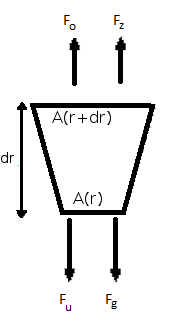
\includegraphics{differential}
	\label{fig:differential}
\end{figure}

Um nun die Zugkraft in einer Höhe $r$ zu bestimmen, lassen wir nun die Höhe unserer Seilabschnitte $dr$ gegen 0 gehen.\\
Für den nächsten Schritt müssen wir voraussetzen, dass A stetig ist. Wir können dies Problemlos tun, indem wir A einfach auf solche Lösungen Einschränken, die stetig sind, da unser Lösungsweg so oder so genau solche A finden wird. Aus der Stetigkeit von $A$ können wir nun für $dr \rightarrow 0$ folgern, dass $A(r)=A(r+dr)$. Somit ergibt sich für die Masse $m_{dr}$ unserer Seilabschnitte die Gleichung \ref{eq:samass}.

\begin{equation}
m_{dr} = A(r) \cdot \varrho \cdot dr
\label{eq:samass}
\end{equation}

Mit dieser Masse können wir nun auch Gleichungen für die Kräfte $F_g$ (\ref{eq:Fg}) und $F_z$(\ref{eq:Fz}) aufstellen:

\begin{align}
F_g &= A(r) \cdot \varrho \cdot g_0 \cdot M_E \cdot \frac{1}{r^2} \cdot dr\label{eq:Fg}\\
F_z &= A(r) \cdot \varrho \cdot r \cdot \omega^2 \cdot dr\label{eq:Fz}
\end{align}

Wir vernachlässigen hierbei den Unterschied zwischen der Höhe $r$ und der Höhe $r+dr$, da $r+dr\rightarrow r$ für $dr \rightarrow 0$.

Die nötige Zugkraft auf der Höhe $r$ ist nun die Summe aller Differenzen der Kräfte $F_g$ und $F_z$, die sich für jeden (infinitesimal kleinen) Seilabschnitt unterhalb der Höhe $r$ ergeben. Diese Summe entspricht genau dem Integral aus Gleichung \ref{eq:taperint}. Die linke Seite der Gleichung ergibt sich sofort aus der Ersetzung von $Z(r)$ durch $\sigma \cdot A(r)$

Ein großer Vorteil dieser Modellierung gegenüber der Formulierung des Problems mit konstanter Querschnittfläche ist, dass sofern unabhängig von den vorkommenden Konstanten Lösungen für diese Integralgleichung existieren, sich ein stabiles Seil für jedes erdenkliche Material konstruieren lässt, wenn auch nur theoretisch. Es sollte offensichtlich sein, dass sich aus der bloßen theoretischen Existenz dieser Lösung noch keine praktische Umsetzbarkeit ergibt.

\subsection{Lösung für Tapering-Modell}

Um die Lösungen der Integralgleichung zu bestimmen, wenden wir zunächst den Fundamentalsatz der Analysis an und formen die Gleichung so zur Differentialgleichung \ref{eq:taperdgl} um.
\begin{equation}
A'(r) \cdot \sigma = A(r) \cdot \varrho \cdot g_0 \cdot M_E \cdot \frac{1}{\tilde{r}^2} - A(r) \cdot \varrho \cdot \omega \cdot \tilde{r}\ d\tilde{r}
\label{eq:taperdgl}
\end{equation}

Dies ist eine nicht autonome gewöhnliche homogene lineare Differentialgleichung 1. Ordnung.

%TODO justify

In der Literatur\cite{PE75} findet man sie auch in der Form \ref{eq:taperdgllit}.

\begin{equation}
A'(r) \cdot \sigma = \varrho \cdot g_E \cdot {r_E}^2 \cdot (\frac{1}{r^2} - \frac{r}{{r_{geo}}^3}) \cdot A(r)\ dr
\label{eq:taperdgllit}
\end{equation}

%TODO justify

Da unsere Differentialgleichung \ref{eq:taperdgl} separierbar ist, können wir sie sehr einfach durch Trennung der Variablen lösen.

%TODO do it

Wir erhalten nun also eine Lösung der Form \ref{eq:tapersolution}

\begin{align}
A(r) &= c_I * e^{\frac{-2\rho \cdot m_E \cdot G - \rho \omega^2 \cdot r^3}{2 r \sigma}}\label{eq:tapersolution}\\
c_I &= A(r_0) \cdot e^{-\frac{-2 c \rho m_E G - \rho \omega^2 r_0^3}{2 r_0 \sigma}}
\end{align}

Analog zur obigen Umformung \ref{eq:taperdgllit} unserer ursprünglichen Differentialgleichung \ref{eq:taperdgl} findet man in der Literatur auch die Lösung \ref{eq:tapersolutionlit}

\begin{equation}
A(r)=A_{geo}*e^\frac{3r_E^2}{2*h*r_{geo}}*e^{\frac{-r_E}{h}*(\frac{r_E}{r}+\frac{r_E*r^2}{2r_{geo}^3})}
\label{eq:tapersolutionlit}
\end{equation}

Basierend auf dieser Lösung lässt sich das so genannte Taperverhältnis bestimmen. Dies ist der Quotient zwischen der Querschnittfläche auf der Erdoberfläche und der 

\begin{equation}
\frac{A}{A_0} = e^\frac{0,776*r_E}{h}
\label{eq:taperratio}
\end{equation}
$h=\frac{\sigma}{\varrho*g_0}$ mit $\sigma$ ist die als konstant(!) gesetzte Belastung. Man erkennt mit zunehmendem $h$ nimmt das Taperverhältnis ab.
Aus Gleichung \ref{eq:taperdgl} folgt, dass die größte Zugkraft am geostationären Orbit auf das Seil wirkt. Dies kann auch daraus geschlussfolgert werden, dass an diesem Punkt zwei gleich große Kräfte in entgegengesetzte Richtungen wirken. Zum einen die Kraft des Seils, das Richtung Erde zieht und zum anderen der Teil des Seils, der vom geostationären Orbit aus von der Erde weg zeigt. Man beachte, dass der geostationäre Orbit genau der Punkt ist, an dem sich die Gravitationskraft der Erde und die Fliehkraft, die auf das Objekt wirkt gegenseitig aufheben, wäre eine Kraft größer, so würde sich das Objekt auf eine andere Umlaufbahn bewegen. Daraus folgt auch, dass die Kraft, die auf den geostationären Punkt wirkt, maximal ist. \\
In Abbildung \ref{fig:Tapering} erkennt man, wie das Taperingverhältnis zunimmt bis zum geostationären Orbit und dann wieder abnimmt. Die Kurve ist nicht symmetrisch, da die Gravitation von der Erde weg mit einem anderen Faktor abnimmt, als sie zur Erde hin zunimmt.
\begin{figure}[!htb]
\centering
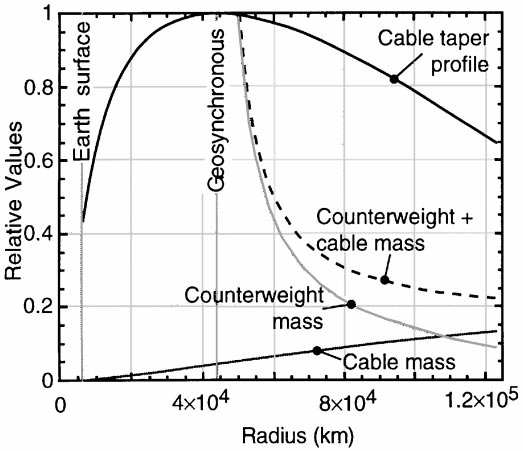
\includegraphics[scale=0.4]{Tapering.png} 
\caption{Kabel Taper Profil, entnommen aus Edwards(2000)\cite{ED00}}
\label{fig:Tapering}
\end{figure}
\\
Vergleicht man die drei Materialien aus dem vorherigen Abschnitt bezüglich ihres Taper Verhältnisses am geostationären Punkt, so erhält man die folgenden Werte:

\begin{itemize}
\item Stahl: \ \ \ \ $\frac{A_{geo}}{A_0} = 5,8 *10^82$
\item Kevlar:\ \ \   $\frac{A_{geo}}{A_0} = 2,71 *10^8$
\item CNT: \ \ \ \ $\frac{A_{geo}}{A_0} = 1,62\ bis\ 8,2 $ 
\end{itemize}

Auf Grund der Größenordnung des Verhältnisses ist die einzige Lösung für die Materialwahl Carbon Nano Tubes, Stahl und Kevlar und andere Materialien haben ein zu großes Taperverhältnis.

\subsection{Modell mit Nutzlast}

%TODO Nutzlast Modell

%TODO Nutzlast Rechnung

\chapter{Implementierung des Modells}
Im nächsten Schritt wollen wir uns mit der Implementierung des mathematische Modells genauer befassen. Hier wird als erster der Code detailliert vorgestellt, um daraufhin die daraus resultierenden Ergebnisse und Zahlen in Verbindung mit der Realität zu bringen. Dies bildet die Grundlage für das letzte Kapitel, in dem weitere Schwierigkeiten dargestellt werden sollen und ein Ausblick in die Zukunft gegeben wird.
\section{Der zugrundeliegende Code}
Die erste Frage, die sich bei einer Implementierung eines mathematischen Modells stellt, ist die Frage nach einer geeigneten Programmiersprache. Hier fällt die Wahl sehr schnell schon auf Python, welche von Grund auf Bibliotheken wie numpy und scipy mit sich bringt. Durch beide Bibliotheken lassen sich zum Beispiel das Bilden von Integralen und die Berechnungen von Exponentialfunktionen leicht umsetzen. 
Im Folgenden stellen wir nun die verschiedenen Abschnitte der Pythonimplementierung vor.\\
Das Ziel unseres Programms ist die Berechnung verschiedener Massen des Aufzugkabels in Abhängigkeit mehrerer Faktoren wie Länge des Kabels, Schnittfläche auf Höhe des Erdradius oder Größe des Sicherheitsfaktors.
 
\lstset{style=mystyle}
\begin{lstlisting}[language=Python, caption=Python Variableninitialisierung]
import math
import scipy.integrate as integrate
import numpy as np
import matplotlib.pyplot as plt

#Initialisiere Konstanten/Variablen
r_E= np.float128(6370000) # in m
r_geo=np.float128(42300000) # in m
H = np.float128(100000000) # in m

w=np.float128(7.29*10**-5) # in 1/s
G =np.float128(6.67*10**-11) #Gravitationskonstante in Nm^2/kg^2
rho=np.float128(1500) # Dichte
sigma=np.float128(100000000000) #Zugfestigkeit irgendwo zwischen 30 und 130 GPa
m_E=np.float128(5.972*10**24) # in kg
s=np.float128(2) #Sicherheitsfaktor, wenn > 1
A_E=np.float128(1.5*10**-7)
A_mehrere = [0.1*10**-7, 0.2*10**-7, 0.3*10**-7, 0.4*10**-7, 0.5*10**-7, 1*10**-7, 1.5*10**-7, 3*10**-7, 10*10**-7, 20*10**-7]

\end{lstlisting}
Als erster Schritt werden die benötigten Konstanten initialisiert. Hierunter fallen der Erdradius \( r_E \), die Entfernung zum geostationären Orbit \( r_{geo} \), die absolute Länge des Seils \( H \), die Winkelgeschwindigkeit der Erde \(\omega \), die Gravitationskonstante \(\ G \), die Zugfestigkeit des potentiell verwendeten Materials \(\varrho \) und die Dichte des Materials \(\sigma \). Als letzte Konstante wählen wir die Schnittfläche \( A_E \) des Seils auf Höhe des Erdradiuses. Letztere Konstante kann später auch als variable angesehen werden, aufgrund von Vereinfachungen von Berechnungen wird dieser Wert aber als Konstante initialisiert, weswegen für spätere Kalkulationen ein Array mit mehreren Werten \( A_E \) befüllt wird.\
Der in Kapitel 3 eingeführte Sicherheitsfaktor wird bei der ersten Initialisierung auf 2 festgelegt. Wir werden später jedoch noch erkennen, dass dies ein äußerst hoher Wert ist und in der Praxis meist kleinere Werte nahe bei Null als sinnvoll erachtet werden können.

\begin{lstlisting}[language=Python, caption=Aufstellen der Funktion zur Berechnung der Schnittfläche] 
def A(r):
  return A_E*np.exp(-(s(-2*rho*m_E*G/2*r_E+rho*w**2*r_E**2)/(2*r_E*sigma)))*np.exp((s*2(rho*m_E*G/r+rho*w**2*r**2)/(2*sigma*r)))
\end{lstlisting}
Die nächste Programmzeile in unserer Implementierung stellt die Formel 
\begin{equation}
A(r)=A_E \cdot e^\frac{-s(-2\varrho m_E G-\varrho\omega^2r_E^2)}{2r_E\sigma} \cdot e^\frac{s(-2\varrho m_E G-\varrho\omega^2r^2)}{2r\sigma}
\end{equation}
dar, welche zu jeder Eingabe die Schnittfläche des Seils in Höhe \( r \) ausgibt. Dies bildet das Kernstück des Programms, worauf deswegen im weiteren Programm immer wieder Bezug genommen wird. Die Herleitung jener Formel wurde bereits in vorangegangenen Kapitel aufgezeigt. Wie anfangs bereits geschildert interessieren wir uns hauptsächlich für die Masse des vorliegenden Kabels. Um diese zu berechnen, machen wir uns folgende Formel zu Nutze[?]:\\
\begin{equation}
m_{Kabel} = \varrho \cdot \int_{r_E}^{H} A(r) dr
\end{equation}
Um das Programm nicht für jeden möglichen Wert \( A_E \) neu starten zu müssen, wurde wie bereits beschrieben ein Array hierfür angelegt, welches in einer for-Schleife durchlaufen und die dazugehörige Masse berechnet wird. Diese wird in einem noch unbefüllten Array gespeichert, welches zuvor initialisiert wurde. Für die Berechnung des Integrals wird die bereits erwähnte Bibliothek scipy verwendet.

\begin{lstlisting}[language=Python, caption=Hinzufügen von Funkionalität]
weights_rope = []

for a in A_mehrere:
  A_E = a
  m_Kabel= integrate.quad(A, r_E, H)
  weights_rope.append(rho*(m_Kabel1[0]))
  
# Gewicht Seil
print("-----Gewicht Seile-----")
print(weights_rope)
  
\end{lstlisting}
Gibt man nun die Werte aus, die in \( m_{Kabel} \) gespeichert worden sind, so erhält man erste Massenwerte. Hierbei ist die Länge des Seils 100000 km lang, die Zugfestigkeit liegt bei 100 GPa und der Sicherheitsfaktor wurde auf 2 gesetzt.\\
\begin{table}[htb]
\centering
\begin{tabular}{|l|r|}

\hline
\( A_E \) in \textmu \( m^2 \) & Gewicht des Seil in kg\\
\hline
0,1	& 5.008\\
0,2	& 10.016\\
0,3	& 15.024\\
0,4	& 20.032\\
0,5	& 25.040\\
1	& 50.080\\
1,5	& 75.119\\
3	& 150.239\\
10	& 500.796\\
20	& 1.001.591\\
\hline
\end{tabular}
\caption{Schnittflächen und Massen des Seils} \label{tab:sometab}
\end{table}\\
Wie man nun an der Tabelle deutlich erkennen kann, verhalten sich die Schnittfläche und das Gewicht des Seils zum Einen natürlich direkt proportional. Zum Anderen steigt das Gewicht linear an, was auch schon an Formel (5.1) klar sichtbar ist. Der erste Teil \( A_E \) bildet bei Festlegung aller anderen Werte die einzige Variable, was aus der Formel eine einfach zu lösende lineare Gleichung macht.\\
Nun gehen wir einen Schritt weiter und wollen den Nutzen des Seils berechnen, was auf das Maximale Gewicht eines Lifters, der am Seil nach oben gezogen werden kann, hinausläuft. Das effektive Gewicht des Lifters mit der Massen \( m_L \) auf der Erdoberfläche ist \( m_L \cdot (g - \omega^2 \cdot r_E) \). Wegen der Zugspannung im Kabel muss diese Gewicht nun von der nach oben gerichteten Kraft \( A_E \cdot \sigma \) entgegengewirkt werden, was zu der Gleichung\\
\begin{equation}
m_L \cdot (g - \omega^2 \cdot r_E) =  A_E \cdot \sigma
\end{equation}
führt, welche nun nach \( m_L \) aufgelöst werden kann und somit die Gleichung (5.4) zur Folge hat, in welcher der Sicherheitsfaktor s bereits berücksichtigt wird:[?]\\
\begin{equation}
m_L =   \frac{A_E \cdot (\sigma - \frac{\sigma}{s})} {(g - \omega^2 \cdot r_E)}
\end{equation}
\\
Es ist nun besonderes Augenmerk auf die Zugfestigkeit \( \sigma \) in Verbindung mit unserem Sicherheitsfaktor s zu legen. Setzt man den Sicherheitsfaktor auf 1, hat dies zu Folge, dass der Term   \((\sigma - \frac{\sigma}{s})\) gleich 0 wird und die maximale Masse des Lifters ebenfalls auf 0 fällt. Diese Erkenntnis wird ebenfalls von der in Formel (5.1) berechneten Schnittfläche unterstützt. Ein Sicherheitsfaktor von 1 bedeutet nämlich genau dies; ein Seil, welches von der Erdoberfläche knapp 100000 km in das Weltall gespannt wird und sich genau selbst hält.
Die Formel (5.4) wird nun ebenfalls der Implementierung hinzugefügt. Hierfür erweitern wir Listing 5.3 zu folgendem Code:\\
\begin{lstlisting}[language=Python, caption=Hinzufügen der Berechnungen zur Ermittlung des max. Gewichts des Lifters]
weights_rope = []
weights_lifter = []
A_geo = []
A_r_vergleich = []
TaperVergleich = []

for a in A_mehrere:
  A_E = a
  m_Kabel= integrate.quad(A, r_E, H)
  weights_rope.append(rho*(m_Kabel1[0]))
  weights_lifter.append((a*(sigma-sigma/s))/((G*m_E/r_E**2)-w**2*r_E))
  A_geo.append(testrun(R_geo))
  TaperVergleich.append(a*(np.exp(0.776*R_e/r_geo))**1)
  
#Gewicht Seil
print("-----Gewicht Seile-----")
print(weights_rope)

#Gewicht Lifter
print("-----Max Gewicht Lifter-----")
print(weights_lifter)

#A_geo
print("-----A_Geo-----")
print(A_geo)
\end{lstlisting}
Zusätzlich interessiert uns noch das Taperverhältnis und die dazugehörige Schnittfläche \( A_geo \) am geostationären Orbit, welche ebenfalls implementiert worden ist. Das Programm wird nun, mit gleichen Werten wie bereits für Tabelle 5.1 verwendet, ausgeführt. \\


\begin{table}[htb]
\centering
\begin{tabular}{|l|c|c|r|}


Höhe des Seils in km & Dichte des Seils in \( \frac{kg}{m^3} \)  & Zugfestigkeit \( \sigma \) in GPA & Sicherheitsfaktor \\
\hline
100000 &	1.500 &	100 & 2\\
& & & \\

\hline
\( A_E \) in \textmu \( m^2 \) & Gewicht des Seil in kg & Max. Gewicht des Lifters in kg & \( A_geo \) in \textmu \( m^2 \) \\

\hline
0,1	& 5.008	& 51,10971746	& 0,428629264\\
0,2	& 10.016	& 102,2194349	& 0,857258527\\
0,3	& 15.024	& 153,3291524	& 1,285887791\\
0,4	& 20.032	& 204,4388699	& 1,714517054\\
0,5	& 25.040	& 255,5485873	& 2,143146318\\
1	& 50.080	& 511,0971746	& 4,286292636\\
1,5	& 75.119	& 766,645762	& 6,429438954\\
3	& 150.239	& 1533,291524	& 12,85887791\\
10	& 500.796	& 5110,971746	& 42,86292636\\
20	& 1.001.591	& 10221,94349	& 85,72585272\\

\hline
\end{tabular}
\caption{Daten des zweiten Durchlaufs} \label{tab:sometab}
\end{table}
\section{Die Ergebnisse der Berechnungen}
Wie auch schon im ersten Durchlauf kann man in Tabelle 5.2 die Linearität sowohl der Masse des Seils, als nun aber auch des maximalen Gewicht des Lifters klar sehen. Das Taperverhältnis von knapp 4,3 ist äußerst gut, hierzu sind aber bereits Erläuterungen in der Arbeit vorgestellt worden.\\
In Tabelle 5.3 sind für einen weiteren Durchlauf bis auf die Änderung der Zugfestigkeit keine Änderungen vorgenommen worden. \( \sigma \) ist testweise auf den bisher angenommenen möglichen Maximalwert von Carbon-Nano-Tubes gesetzt worden, welche bei 300 GPa liegt. Dies ist natürlich weit von der Realität entfernt, soll aber nochmals verdeutlichen, welche starken Auswirkungen das Material des Seils auf das Modell und die Realisierbarkeit des Projekts hätte.

\begin{table}[htb]
\centering
\begin{tabular}{|l|c|c|r|}


Höhe des Seils in km & Dichte des Seils in \( \frac{kg}{m^3} \)  & Zugfestigkeit \( \sigma \) in GPA & Sicherheitsfaktor \\
\hline
100000 &	1.500 &	300 & 2\\
& & & \\

\hline
\( A_E \) in \textmu \( m^2 \) & Gewicht des Seil in kg & Max. Gewicht des Lifters in kg & \( A_geo \) in \textmu \( m^2 \) \\

\hline
0,1	&2.135	&153,3291524&	0,162440359\\
0,2	&4.269	&306,6583048	&0,324880717\\
0,3	&6.404	&459,9874572	&0,487321076\\
0,4	&8.538&	613,3166096	&0,649761434\\
0,5	&10.673&	766,645762&	0,812201793\\
1	&21.346&	1533,291524&	1,624403585\\
1,5	&32.019&	2299,937286&	2,436605378\\
3	&64.037&	4599,874572&	4,873210756\\
10	&213.457&	15332,91524&	1,624403585\\
20	&426.915&	30665,83048	&3,248807171\\

\hline
\end{tabular}
\caption{Daten des dritten Durchlaufs} \label{tab:sometab}
\end{table}

Man kann außerdem erkennen, dass auch unsere Berechnungen das bestmögliche Taperverhältnis von gut 1,6 als Ergebnis bekommen, welches in Kapitel 2 näher erläutert worden ist. Bisher haben wir uns jedoch ausschließlich darauf fokussiert, einzelne Werte im Exponetialteil der Gleichung zu ändern und dabei alle anderen Variablen als Konstanten zu betrachten, was zu der Linearität der Ergebnisse geführt hat. Daher wollen wir nun in der abschließenden Rechnung nicht den linearen Faktor \( A_E \), sondern vielmehr den eingeführten Sicherheitsfaktor \( s \) als Variable ansehen. Der Faktor  \( A_E \) soll nun als Konstante den Wert 1 cm annehmen. Da diese Berechnungen nicht ohne Weiteres mit der aktuellen Implementierung getätigt werden können, muss der Code um Folgendes erweitert werden:

\begin{lstlisting}[language=Python, caption=Berechnungen für konstante Schnittfläche]
#Berechnung Gewichte mit A_E fest
for s in sicherheit:
  sigma=np.float128(100000000000)
  sigma = sigma/s
  m_Kabel= integrate.quad(A, r_E, H)
  weights_rope_dif.append(rho*(m_Kabel[0]))
  weights_lifter_dif.append((A_E*(sigma-sigma/s))/((G*m_E/r_E**2)-w**2*r_E))
  
#Gewicht Seil mit versch Sicherheitsfaktoren
print("-----Gewicht Seile-----")
print(weights_rope_dif)

#Gewicht Lifter mit versch Sicherheitsfaktoren
print("-----Max Gewicht Lifter-----")
print(weights_lifter_dif)
\end{lstlisting}

Hier wird schlichtweg der Sicherheitsfaktor neu angepasst und die berechneten Werte in ein Array gespeichert, welches am Ende ausgegeben wird. Die daraus folgenden Daten in Tabelle 5.4 lasen nun klar erkennen, dass der Sicherheitsfaktor, wie auch angenommen, exponentielle Auswirkungen auf das Gewicht des Seils und logarithmische Auswirkungen auf das maximale Gewicht des Lifters hat.

\begin{table}[htb]
\centering
\begin{tabular}{|l|c|c|r|}


Höhe des Seils in km & Dichte des Seils in \( \frac{kg}{m^3} \)  & Zugfestigkeit \( \sigma \) in GPA &  \\
\hline
100000 &	1.500 &	100 & \\
& & & \\

\hline
\( A_E \) in \textmu \( m^2 \) & Sicherheitsfaktor \( s \)& Gewicht des Seil in kg & Max. Gewicht des Lifters in kg \\

\hline
1	&1,01	&26539,04125	&10,12073613\\
1	&1,1	&28104,35585	&92,92675903\\
1	&1,2	&29955,237	&170,3657249\\
1	&1,5	&36294,92424	&340,7314498\\
1	&2	&50079,56659	&511,0971746\\
1	&3	&95968,39224	&681,4628995\\
1	&4	&185271,5471	&766,645762\\
1	&5	&359894,4672	&817,7554794\\
1	&10	&10641402,96	&919,9749144\\
1	&20	&11237452274	&971,0846318\\
\hline
\end{tabular}
\caption{Daten des dritten Durchlaufs} \label{tab:sometab}
\end{table}

\begin{figure}[htb]
    \subfigure[exponentielle Auswirkung auf das Gewicht des Seils]{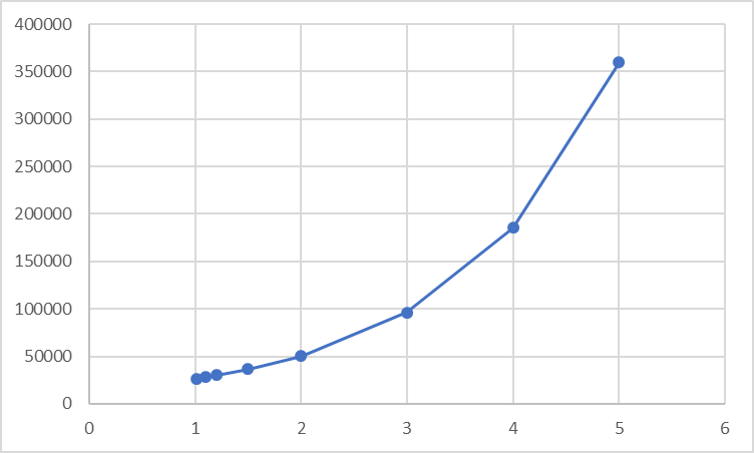
\includegraphics[width=0.49\textwidth]{exponentiell.png}} 
    \subfigure[logarithmische Auswirkung auf das max. Gewicht des Lifters]{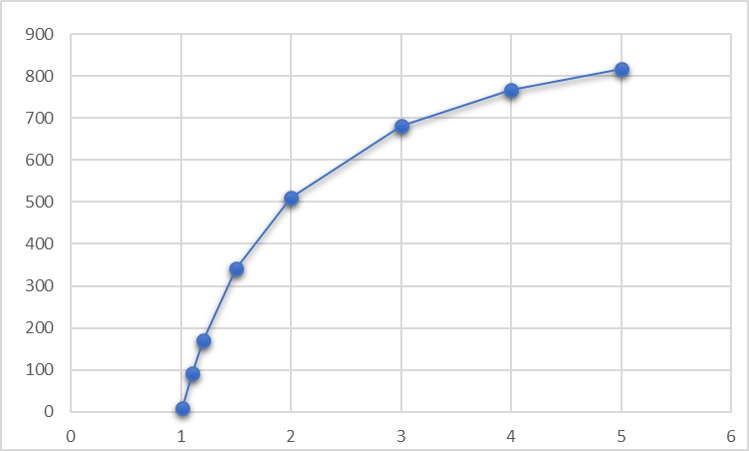
\includegraphics[width=0.49\textwidth]{logarithmisch.png}} 
\caption{Auswirkung der Änderungen des Sicherheitsfaktors \( s \)} 
\end{figure} 

Wie man nun vor allem aus Tabelle 5.4 und Abbildung 5.1 herauslesen kann, wir nicht sofort ersichtlich, welcher Sicherheitsfaktor \( s \)  in Kombination mit welcher Schnittfläche \( A_E \) zu wählen ist, um eine bestmögliche Kombination der drei Faktoren zu bekommen. Eine genauere Betrachtung solcher Fragestellungen und der aufgezeigten Ergebnisse soll nun im letzten Abschnitt der Arbeit stattfinden.  


\bibliography{mybib}{}
\bibliographystyle{plain}


\appendix
\chapter{xxx}
\section{xxx}



\end{document}
